\chapter{Transport domain analysis}

In this chapter, we will analyze two variants of the Transport domain: sequential and temporal. To do this, we will describe a system we developed for the analysis
and development of planners for Transport, describe and analyze the datasets
used for devising experiments, and discuss the properties of Transport
that will aid us in developing better quality planners.

\section{TransportEditor -- A Transportation Planning System}

To aid us and others in studying transportation planning,
we have developed \textit{TransportEditor} --- a system for creating and visualizing transportation problems and plans.

Specifically, TransportEditor aims to be a problem editor and plan visualizer for the Transport domain (and its variants). It is an intuitive and cross-platform graphical desktop application (Figure~\ref{fig:transporteditor-screenshot})
written in Java.

It allows the user to create a planning session, where they
select a Transport domain variant, load a problem instance from PDDL (Section~\ref{pddl}) or create a new one from scratch.
The road network of the problem is automatically laid out and visualized for the user as a graph with locations as nodes and roads as edges.
Users can then tweak the layout, make changes to vehicle and package properties
and export the problem or domain back into PDDL.

They can also select an external planner
referencing its executable file, or select one of the built-in planners and try to solve
the loaded problem using the selected planner. Internal and external plan validators, like VAL \citep{Howey2003}, can also be selected to verify plans are correct.
Once plans are loaded and verified, it will let the user see a list of actions
in the plan, or plot a Gantt chart (useful for observing concurrent actions in temporal domain variants).

The best feature of TransportEditor is the option of tracing plans. We can select
any action, specify an exact time point or just step through the actions in order and
the road network on the left will display the current state of the problem, as if
all actions before the current point were applied to the start state.
It is possible to do all of this, and more, without ever leaving the TransportEditor user interface.

TransportEditor will help researchers working on this domain fine-tune their planners; they can visualize the various corner cases their planner fails to handle, step through the generated plan and find the points where their approach fails.
A secondary motivation is to be able to test approaches for creating plans for the domain.
For screenshots of typical TransportEditor usage, see the attached \nameref{transport-editor-screenshots}.

\begin{figure}[tbp]
\begin{center}
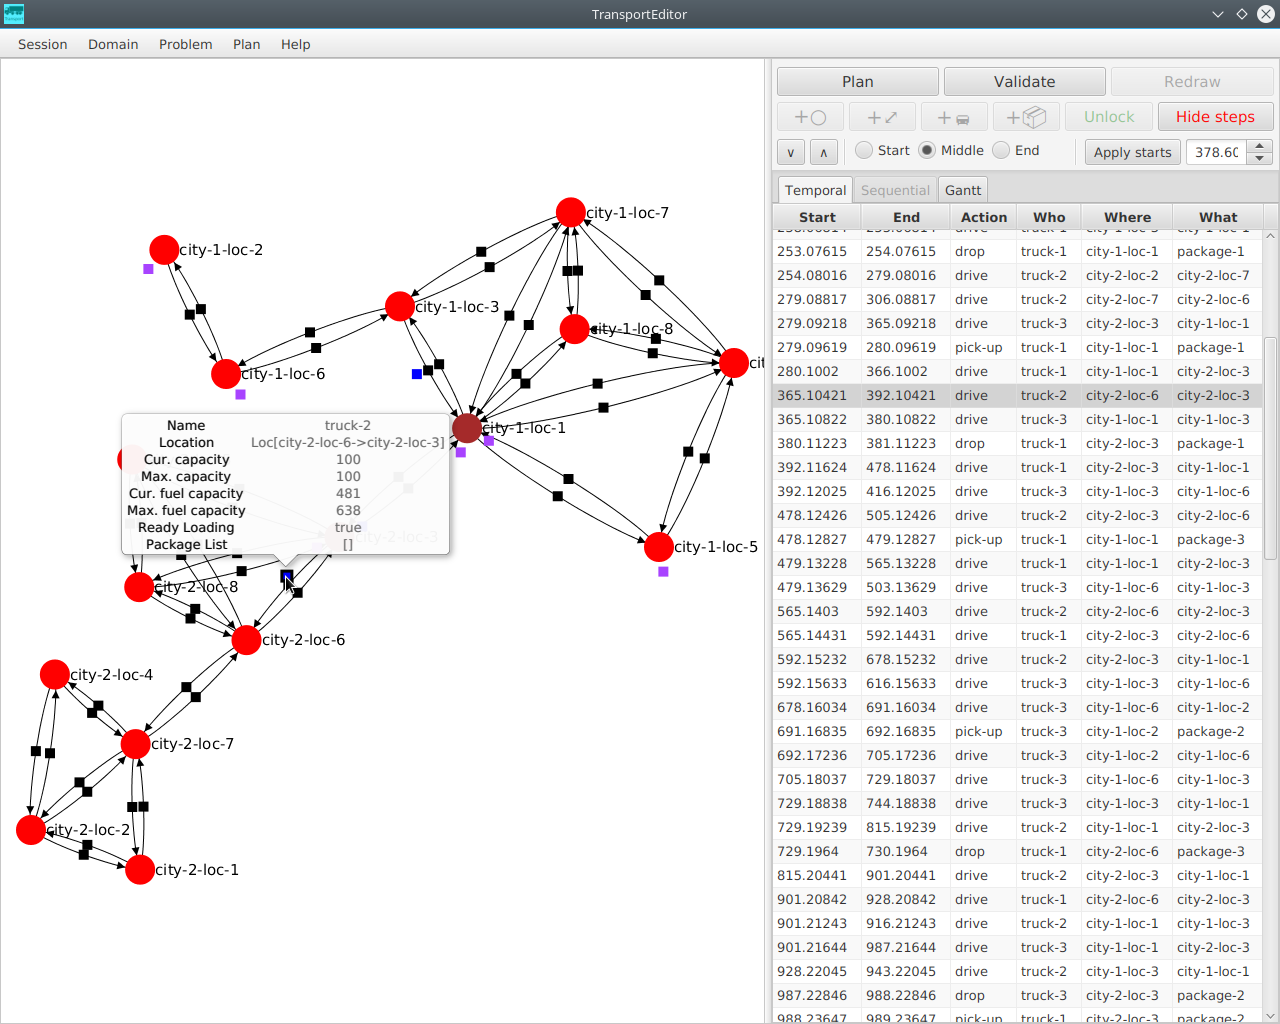
\includegraphics[width=0.9\textwidth]{../img/transporteditor_temporal}
\end{center}
\caption{Screenshot of a user tracing actions of a plan for a smaller temporal problem in TransportEditor.}
\label{fig:transporteditor-screenshot}
\end{figure}

The basic user workflow of TransportEditor consists of the following steps:
\begin{itemize}
\item Selecting which formulation of the Transport domain they want to work with or create their own variant;
\item Loading the PDDL or creating their own problem of the given domain. TransportEditor then visualizes the given graph as good as it can;
\item Iterating among the following options:
\begin{itemize}
\item Loading a planner executable and letting TransportEditor run the planner on the loaded problem instance for a given time (the user can cancel anytime),
then loading the resulting plan;
\item Possibly loading a pre-generated plan;
\item Stepping through the individual plan actions and letting TransportEditor visualize them.
The user can step forward and backward in the plan and inspect each action result in great detail;
\item Editing the graph: adding/removing/editing the location or properties of vehicles, packages, roads, locations and possibly petrol stations;
\item Saving the currently generated plan;
\item Saving the problem;
\item Saving the domain (exporting to a PDDL file).
\end{itemize}
\item Saving and closing the currently loaded problem. Exit the application or go back to the first step.
\end{itemize}

TransportEditor is a part of this thesis and you can find it on the attachment CD (see the attached \nameref{cd-contents} for more information). Both the \nameref{transporteditor-user-manual},
the \nameref{transporteditor-developer-manual}, and the \nameref{transporteditor-developer-javadoc} are attached to this thesis in a digital format, offering guidance when
using the program and providing an in-depth description.














\section{Transport domain analysis}

In this section, we will delve more deeply into the Transport domain and try to analyze its features.
We will describe the problem instances that have been used in the IPC and discuss potential
heuristics and approaches to creating plans for these problems.

\TODO{mention Logistics, Depots, and DriverLog}

\subsection{Does domain knowledge make Transport easy to solve?}

When domain-independent planners solve a sequential Transport problem,
they face a harder task than our planners that have domain knowledge ahead of time.
Deciding whether a plan of a given length exists is, in the case of Transport,
an NEXPTIME-complete task \citep{Ghallab2004}[Section~3.4].
That does not mean domain knowledge makes Transport easy. We will now show
that even the sequential variant of Transport is NP-hard.

\begin{thm}
The problem of finding an optimal plan for an undirected connected graph in the sequential
Transport domain is NP-hard. \TODO{Formulate better and revise proof}
\end{thm}
\begin{proof}
It is not evident if the problem is in NP: if we get a plan, there is no straightforward
way of verifying whether it is optimal.

We will now show that we can reduce an NP-complete problem to our problem in polynomial time,
hence proving that all NP-complete problems are reducible to our problem,
and therefore, our problem is NP-hard.

As proven by \citet{Karp1972}, the problem of existence of a Hamilton circuit (HC) in a (directed or undirected) graph is NP-complete. We will show that we are able to transform the HC problem into a sequential Transport problem.

Given an undirected graph $G$, the solution to HC is a cycle through all the nodes of $G$,
without visiting any single node twice.
We can use the same graph to model a Transport problem instance.
The problem will contain only one vehicle of capacity $n-1$,
where $n = |G|$, the number of nodes in the graph.

We will co-locate $n-1$ packages with the vehicle at any predetermined graph vertex $l \in G$.
One package $p'$ will be located elsewhere, at $l' \in G,\, l \neq l'$.
Each package positioned at $l$ will have a different target than the other packages at $l$
and none of the targets will be $l$. The package at $l'$ will have the original node $l$
as its target. We will set all road lengths to $1$. 

An optimal plan for the designed translation has a total cost of at least $3n$.
Any plan for this problem has to have at least $n$ \verb+drive+ actions, because
there is a package to be delivered to every node, and the graph has $n$ nodes.
Because it has to move $n$ packages, at least $n$ \verb+pick-up+ and $n$ \verb+drop+
actions are needed. The costs of all actions are 1.
We conjecture that an HC exists if and only if an optimal and valid plan visits each vertex only once.

First, we prove the forward implication. Assume an HC exists and the optimal plan visits at least one node twice. We can now construct a plan with a lower total cost than the optimal plan: first, pick up all the $n-1$ co-located packages, then drive along the HC. At each
visited node, drop the package that has this node as its destination. If we are at $l'$,
pick up the package $p'$. The plan is trivially valid, as it delivers all packages
and the vehicle never over-reaches its capacity. Also, its total cost is $3n$
(the length of the HC is $n$, which implies $n$ drive actions) and for every of the $n$ packages, we do exactly one \verb+pick-up+ and exactly one \verb+drop+. Hence, the plan
is optimal and visits each vertex only once.

Now, assume an HC does not exist. If the found optimal plan only visits each node once,
we can look at the source locations of all \verb+drive+ actions and the target
location of the last \verb+drive+ action. They constitute a path through the graph on which a node never repeats and the path starts and finishes at the same node.
Hence, we have constructed a HC.
\end{proof}

\subsection{Domain features}

\TODO{insights, degenerate cases, etc.}



















\section{Datasets}

We have acquired several datasets from previous runs of the IPC which we will use to test our planners.
Table~\ref{tab:ipc-datasets} provides an overview of the distinct datasets, their associated IPC competition, track at the competition and the formulation used (descriptions of the tracks in hyperlinks).

\begin{table}[tb]
\begin{tabular}{c||ccc}
\textbf{Dataset} & \textbf{Competition} & \textbf{IPC Track} & \textbf{Formulation} \\ 
\hline
\hline
netben-opt-6 & IPC-6 & \href{http://icaps-conference.org/ipc2008/deterministic/NetBenefitOptimization.html}{Net-benefit: optimal} & Numeric \\ 
seq-opt-6 & IPC-6 & \href{http://icaps-conference.org/ipc2008/deterministic/SequentialOptimization.html}{Sequential: optimal} & STRIPS \\ 
seq-sat-6 & IPC-6 & \href{http://icaps-conference.org/ipc2008/deterministic/SequentialSatisficing.html}{Sequential: satisficing} & STRIPS \\ 
tempo-sat-6 & IPC-6 & \href{http://icaps-conference.org/ipc2008/deterministic/TemporalSatisficing.html}{Temporal: satisficing} & Temporal \\ 
\hline
seq-agl-8 & IPC-8 & \href{https://helios.hud.ac.uk/scommv/IPC-14/seqagi.html}{Sequential: agile} & STRIPS \\ 
seq-mco-8 & IPC-8 & \href{https://helios.hud.ac.uk/scommv/IPC-14/seqmulti.html}{Sequential: multi-core} & STRIPS \\ 
seq-opt-8 & IPC-8 & \href{https://helios.hud.ac.uk/scommv/IPC-14/seqopt.html}{Sequential: optimal} & STRIPS \\ 
seq-sat-8 & IPC-8 & \href{https://helios.hud.ac.uk/scommv/IPC-14/seqsat.html}{Sequential: satisficing} & STRIPS \\ 
\end{tabular}
\caption{Transport datasets from the IPC.}
\label{tab:ipc-datasets}
\end{table}

Short descriptions of the various tracks and subtracks can be found in the rule pages of IPC-6\footnote{\url{https://helios.hud.ac.uk/scommv/IPC-14/rules.html}}
and the rule pages of IPC-8\footnote{\url{http://icaps-conference.org/ipc2008/deterministic/CompetitionRules.html}}.
Unfortunately, we weren't able to acquire the datasets for IPC-7, as the Subversion repository\footnote{\url{http://www.plg.inf.uc3m.es/ipc2011-deterministic/Domains.html}} that promises to contain them is unavailable.

\subsection{Discussion of original competition results}

\TODO{re-read and refactor after moving here}

In the updated results of the seq-sat track of IPC 2008\footnote{\url{http://icaps-conference.org/ipc2008/deterministic/Results.html}} published after the competition,
the overall winner \textit{lama} (a Fast-Downward \TODO{ref} planner configuration)
was hands-down the best planner on the sequential Transport domain, winning
with a total quality of $28.93/30$, where all other planners had less than $20/30$.
Only 5 problem instances were solved suboptimally by \textit{lama}.
\textit{Quality} is calculated for a given planner and problem $p$
as $$\frac{\mt{total-cost}(\mt{planner}(p))}{\mt{total-cost}(BEST)},$$ where the results called $BEST$
are precalculated outside of the competition environment, or the best result of a planner in the competition, depending on which plan has a lower total cost. The quality is, therefore, a number between $0$ and $1$. The total quality is calculated as the sum of qualities on all problem instances.

As mentioned, we were not able to gather data from the IPC 2011,
hence the results cannot be meaningfully interpreted.
The competition featured 20 sequential Transport problems,
with 4 planners achieving a total quality of more than $15/20$.

In the seq-sat track of IPC 2014, the winner on the Transport domain
was without a doubt the \textit{Mercury} planner, achieving
a stunning $20/20$ total quality. Even more interesting is the fact that
the runner-up \textit{yahsp3-mt} achieved a score of $10.74/20$
and all other planners achieved sub $10/20$ total quality.
The IPC 2014 used different problem instances than the IPC 2008
and we will test our approaches on both datasets.

The temporal variant of Transport was only used in IPC 2008.
Planners that entered that competition did not cope well with the domain
--- only two \TODO{base?} planners were able to produce at least one plan
for any problem. Additionally, only the simple problem (\verb+p01+) was solved
optimally by any planner. The best total quality was only $7.5/30$, achieved by
\textit{sgplan6}. No other domain in the temporal track had a lower best total quality
than Transport, which, assuming reasonably generated problem instances, hints
at Transport being one of the harder domains for domain-independent temporal planners.

\subsection{Problem instances}

\TODO{specific problems we will be using}

\subsection{Problem features}

\TODO{features and peculiarities of the problem instances}
















\section{Formulating Transport as a CSP}\label{csp-formulation}

\TODO{intro}

\subsection{Na{\"{i}}ve formulation}

We will now formulate a sequential Transport (Section~\ref{transport-strips}) problem as a CSP (Section~\ref{csp}) using the na{\"{i}}ve encoding provided in \citet[Section~8.3]{Ghallab2004}.
However, using that strategy, our problems ``blow up'' in size --- as is expected due
to the different complexities of planning versus solving CSPs \citep[Section~8.3.2]{Ghallab2004}. To visualize the difference in our case, we have constructed a state space estimation table (Table~\ref{tab:csp-trivial}) for conversions of two sample sequential Transport problems.

\begin{table}[tb]
\begin{center}
\begin{tabular}{l||rr}
\textbf{Features / estimates} & \textbf{p01} & \textbf{p20} \\ 
\hline 
\hline 
\textbf{Best known plan length} & 6 & 351 \\ 
\textbf{Vehicles} & 2 & 4 \\ 
\textbf{Vehicle variables} & 14 & 1 408 \\ 
\textbf{Packages} & 2 & 20 \\ 
\textbf{Package variables} & 14 & 7 040 \\ 
\textbf{Locations} & 5 & 60 \\ 
\textbf{Roads} & 12 & 256 \\
\textbf{Max capacity} & 4 & 4 \\ 
\hline
\textbf{Ground Drive actions} & 168 & 360 448 \\ 
\textbf{Ground PickUp actions} & 140 & 1 689 600 \\ 
\textbf{Ground Drop actions} & 140 & 1 689 600 \\ 
\hline 
\textbf{Planning variables total} & 48 & 10 207 \\ 
\textbf{Grounded actions total} & 448 & 1 189 838 848 \\ 
\textbf{Search Space Estimate} & $\approx 1.1 \cdot 10^{52}$ & $\approx 1.4 \cdot 10^{27 952}$ \\ % https://www.wolframalpha.com/input/?i=(245120%5E351)+*+4%5E1408+*+60%5E1408+*+1468%5E7040
\end{tabular}
\end{center}
\caption[Search space approximations for a na{\"{i}}ve CSP encoding.]{CSP Search space approximations for the \textit{p01} and \textit{p20} problems from the \textit{seq-sat} track of IPC 2008, using the general and domain-independent encoding from \citet[Section~8.3]{Ghallab2004}.}
\label{tab:csp-trivial}
\end{table}

The first section of the table (rows 1--7) contains problem-specific constants.
The two calculated values in that section, \textit{Vehicle variables} and \textit{Package variables} are the amounts of variables generated for the respective
object by grounding it for every intermediate plan state (before and after applying an action). Therefore, the value is equal to the number of vehicles/packages of the problem
multiplied by the set plan length $+ 1$ (each state corresponds to the state before applying an action + the last state).

In the second section (rows 8--10), we estimate the number of ground actions
Step 1 from \citet[Section~8.3.1]{Ghallab2004} will generate.
We calculate the number of \pickup{} and \drop{} actions the CSP encoding will generate
as $$(\mt{length(plan)} + 1) \cdot \mt{\#vehicles} \cdot \mt{\#locations} \cdot \mt{\#packages},$$
effectively counting all ground planning operators of the problem. Similarly,
the number of \drive{} actions is calculated as
$$(\mt{length(plan)} + 1) \cdot \mt{\#vehicles} \cdot \mt{\#roads},$$
which is more efficient than the na{\"{i}}ve way of
counting all
$$(\mt{length(plan)} + 1) \cdot \mt{\#vehicles} \cdot \mt{\#locations}^2$$
actions.

As we can see from the third section of the table, the number of variables
(planning variables and ground actions) is not extremely high
--- the problem is that the variables have very large domains,
which makes the CSP problem exponentially larger \citep[Section~8.3.2]{Ghallab2004}.
We calculated the \textit{Search Space Size Estimate} (SSE) as
\begin{align*}
\mt{SSE} =\; &\mt{\#ground\_actions}^{l-1} & \textit{\footnotesize select ground actions for the plan}\\
&\cdot \mt{\#capacities}^{l \cdot \mt{\#vehicles}} & \textit{\footnotesize select capacities for vehicle variables}\\
&\cdot \mt{\#locations}^{l \cdot \mt{\#vehicles}} & \textit{\footnotesize select locations for vehicle variables}\\
&\cdot (\mt{\#locations} + \mt{\#vehicles})^{l \cdot \mt{\#pkg}}, & \textit{\footnotesize select locations/vehicles for package variables}
\end{align*}
where we set $l := \mt{length(plan) + 1}$.
For comparison to the SSEs in the last table row, 
the estimated number of atoms in the universe is generally estimated to be about $4 \cdot 10^{80}$.

\subsection{Domain-dependent formulation}\label{csp-custom-repr}

\TODO{domain-dep formulation, note the shadow variable overhead}
\TODO{New cap represents advantages: memory while keeping the same expressive power. Reduction only in state vars}


\begin{table}[tb]
\begin{center}
\begin{tabular}{l||rr}
\textbf{Features / estimates} & \textbf{p01} & \textbf{p20} \\ 
\hline 
\hline 
\textbf{Best known plan length} & 6 & 351 \\ 
\textbf{Vehicles} & 2 & 4 \\ 
\textbf{Vehicle shadow vars} & 14 & 1 408 \\
\textbf{Packages} & 2 & 20 \\ 
\textbf{Package shadow vars} & 14 & 7 040 \\
\textbf{Locations} & 5 & 60 \\ 
\textbf{Roads} & 12 & 256 \\
\textbf{Max capacity} & 4 & 4 \\ 
\hline
\textbf{Ground Drive actions} & 24 & 1024 \\ 
\textbf{Ground PickUp actions} & 20 & 4800 \\ 
\textbf{Ground Drop actions} & 20 & 4800 \\ 
\hline 
\textbf{Planning variables total} & 48 & 10 207 \\ 
\textbf{Grounded actions in step} & 64 & 10 624 \\ 
\textbf{Action type orderings} & 2 187 & $\approx 8.8 \cdot 10^{167}$ \\ 
\textbf{Search Space Estimate} & $\approx 1.5 \cdot 10^{14}$ & $\approx 2.0 \cdot 10^{637}$ \\
\end{tabular}
\end{center}
\caption[Search space approximations for a domain-dependent CSP encoding.]{CSP Search space approximations for the \textit{p01} and \textit{p20} problems from the \textit{seq-sat} track of IPC 2008, using a custom domain-dependent CSP encoding for Transport sequential.}
\label{tab:csp-custom}
\end{table}

Using the domain-dependent encoding specified previously, we are now able to construct
a search space estimate table for the same Transport problems (Table~\ref{tab:csp-custom}). While the table rows look similar, sections 2 and 3 are calculated
differently. The ground action counts in section 2 are not multiplied by $\mt{length(plan)} + 1$
as done previously, because we only represent them once, not at every plan state.
The total number of grounded actions is the same, but they are not explicitly represented as variables. The Search Space size Estimate is therefore calculated differently:
\begin{align*}
\mt{SSE} =\; &3^{\mt{length(plan)} + 1} & \textit{\footnotesize select the action type of each action}\\
&\cdot \mt{\#ground\_actions}^{l-1}. & \textit{\footnotesize select the specific ground action}
\end{align*}
For comparison to the na{\"{i}}ve encoding SSEs which going from the p01 problem to the p20 grow by a logarithmic factor of approximately $538$,
whereas the domain-dependent ones only grow by approximately $46$,
which is a huge improvement.

Given the search space reduction, we will attempt to use this representation
for constructing a CSP-based planner in Section~\ref{csp-approach}.
